\section{Configuración de Equilibrio 1}Describan brevemente la primera configuración de equilibrio, considerando la cantidad de masas suspendidas, la disposición de los dinamómetros y los ángulos seleccionados.\begin{table}[h!]
\centering
\begin{tabular}{|c|c|c|}
\hline
\textbf{Fuerza} & \textbf{Módulo ($F \pm \delta F$)} & \textbf{Ángulo ($\theta \pm \delta \theta$)} \\ \hline
$F_1$ & & \\ \hline
$F_2$ & & \\ \hline
$F_3$ & & \\ \hline
\end{tabular}
\caption{Medición directa e indirecta de módulos y ángulos para la Configuración 1.}
\label{tab:config1-mediciones}
\end{table}Los datos recolectados de esta configuración fueron registrados en la Tabla \ref{tab:config1-mediciones}. La representación gráfica de los vectores de esta configuración se puede ver en la Fig. \ref{fig:config1-vectores}.\begin{figure}[h!]
\centering
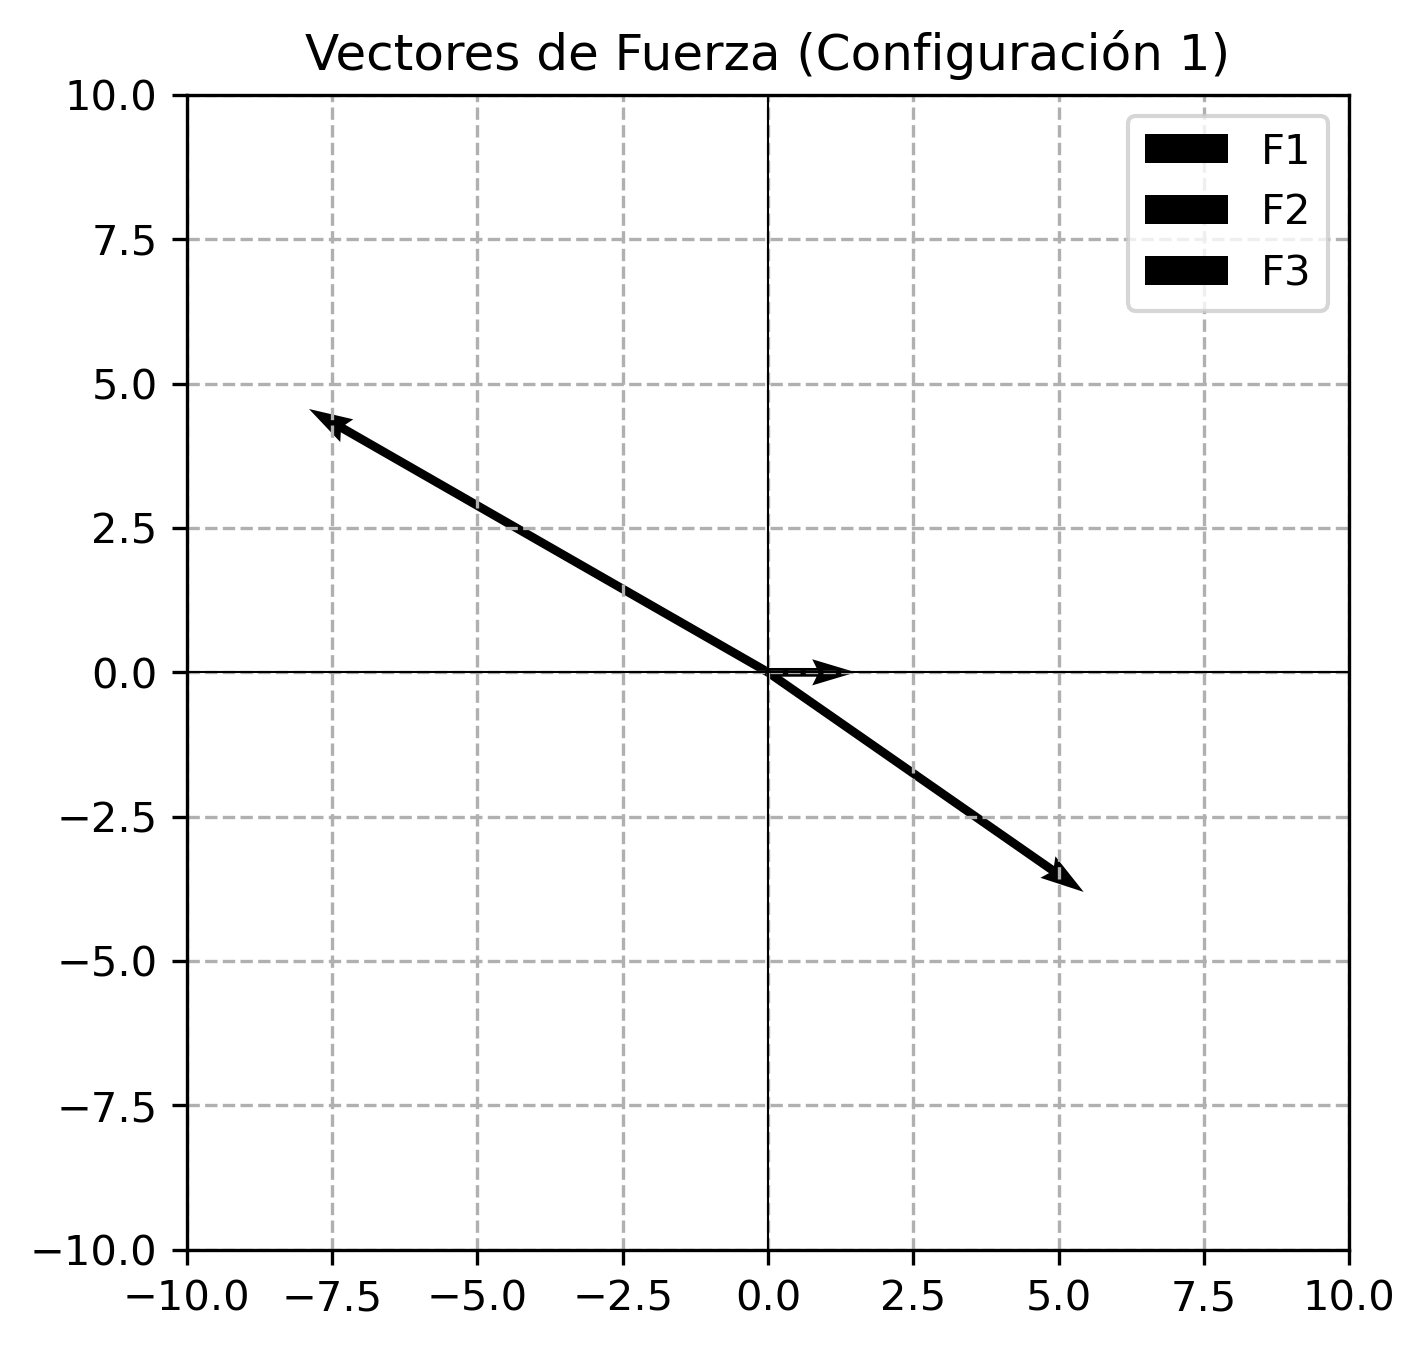
\includegraphics[width=0.4\textwidth]{config1-vectores.png}
\caption{Representación en el sistema de referencia de los vectores $\vec{F}_1$, $\vec{F}_2$ y $\vec{F}_3$ (Configuración 1).}
\label{fig:config1-vectores}
\end{figure}El módulo de $\vec{F}_1$ corresponde al peso de la masa, calculado como $F_1 = mg$. Para obtener $\delta F_1$, se realizó propagación de error.
\begin{equation*}
F_1 = mg = \dots
\end{equation*}
\begin{equation*}
\delta F_1 = \sqrt{\left(\frac{\partial F}{\partial m} \Delta m \right)^2 + \left(\frac{\partial F}{\partial g} \Delta g \right)^2} = \dots
\end{equation*}\subsection{Suma gráfica}La suma gráfica de los vectores se puede ver en la Fig. \ref{fig:config1-poligono}.\begin{figure}[h!]
\centering
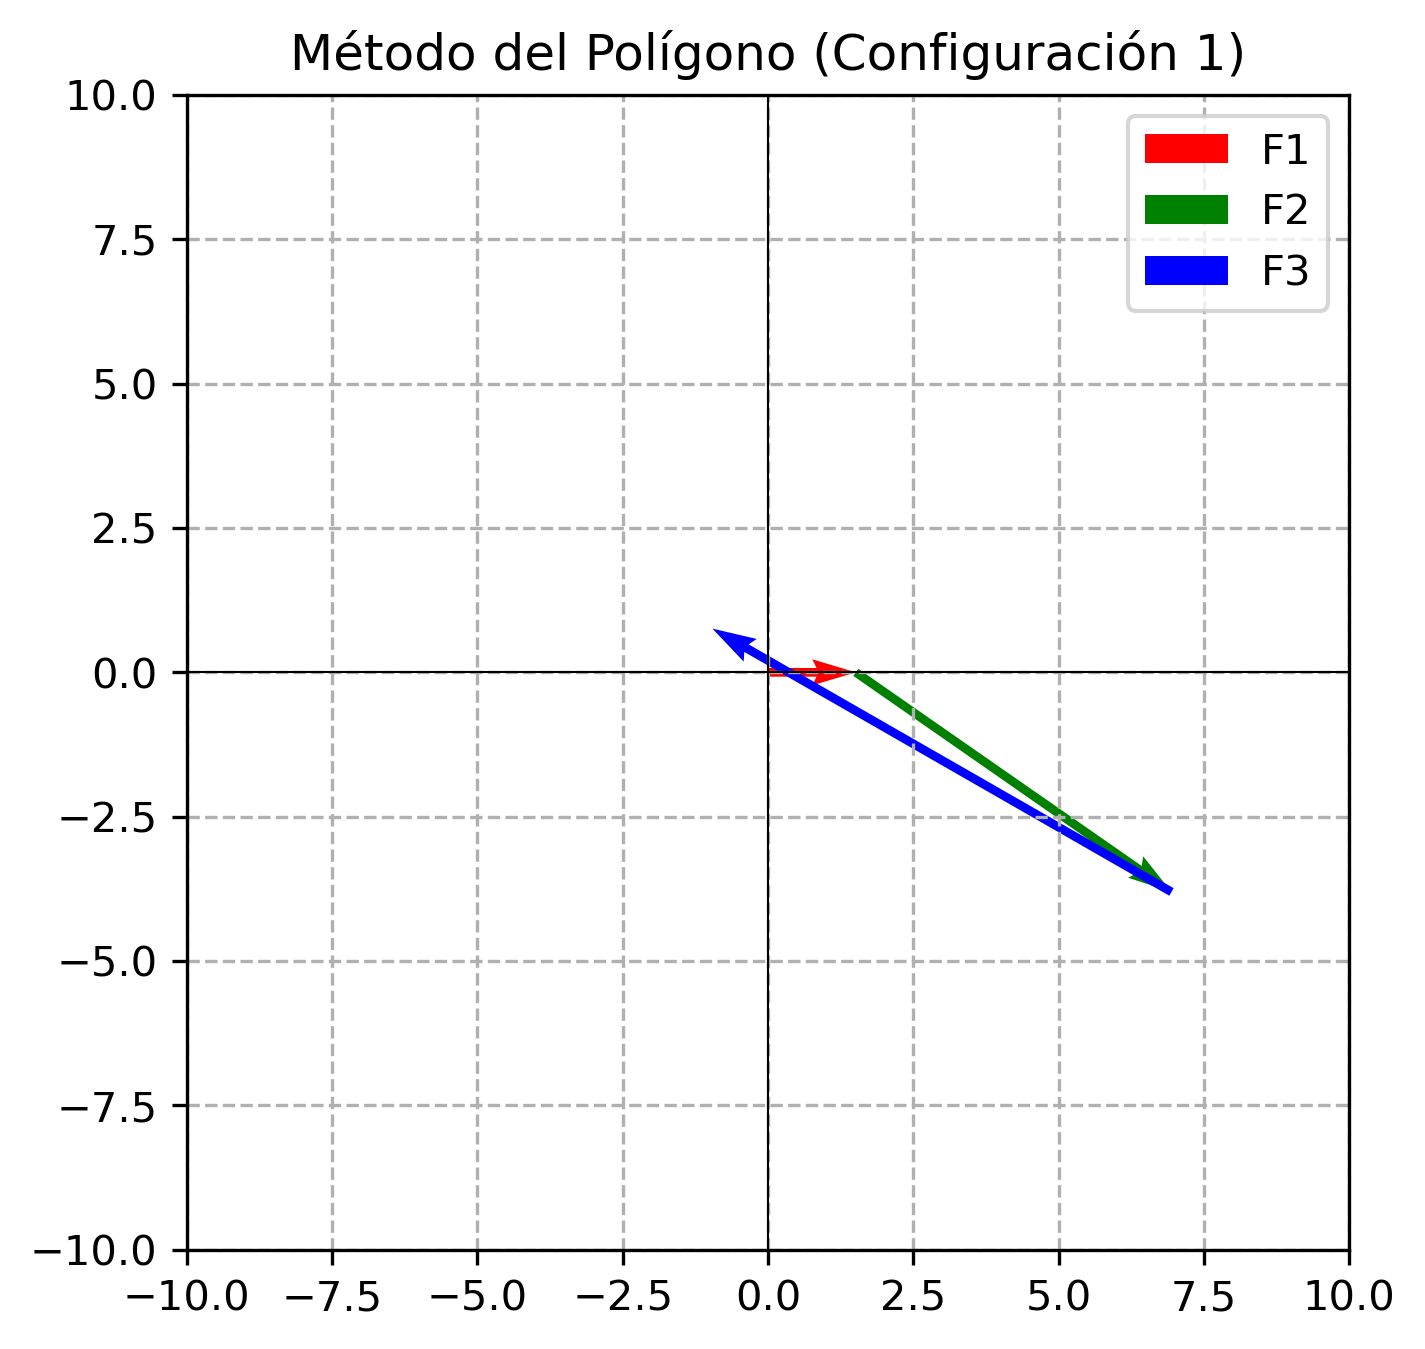
\includegraphics[width=0.4\textwidth]{config1-poligono.png}
\caption{Suma gráfica mediante el método del polígono para la Configuración 1.}
\label{fig:config1-poligono}
\end{figure}Comenten cualitativamente si el polígono se cierra correctamente o si existe alguna discrepancia gráfica visible.\subsection{Suma analítica}Los vectores de la Configuración 1 separados en sus componentes están registrados en la Tabla \ref{tab:config1-componentes}.\begin{table}[h!]
\centering
\begin{tabular}{|c|c|c|}
\hline
\textbf{Fuerza} & $F_x \pm \Delta F_x\,\mathrm{(N)}$ & $F_y \pm \Delta F_y\,\mathrm{(N)}$ \\ \hline
$F_1$ & & \\ \hline
$F_2$ & & \\ \hline
$F_3$ & & \\ \hline
\end{tabular}
\caption{Componentes cartesianas e incertidumbres absolutas para la Configuración 1.}
\label{tab:config1-componentes}
\end{table}Sumando estas componentes, el vector resultante es:\begin{equation*}
\vec{R}_{\mathrm{exp, 1}} = (R_x \pm \Delta R_x),\uveci + (R_y \pm \Delta R_y),\uvecj = (\dots \pm \dots),\uveci + (\dots \pm \dots),\uvecj,\mathrm{N}
\end{equation*}\subsection{Comparación de los resultados}La Fig. \ref{fig:grafico-error-1} muestra la comparación gráfica entre la predicción teórica y el resultado experimental.\begin{figure}[h!]
\centering
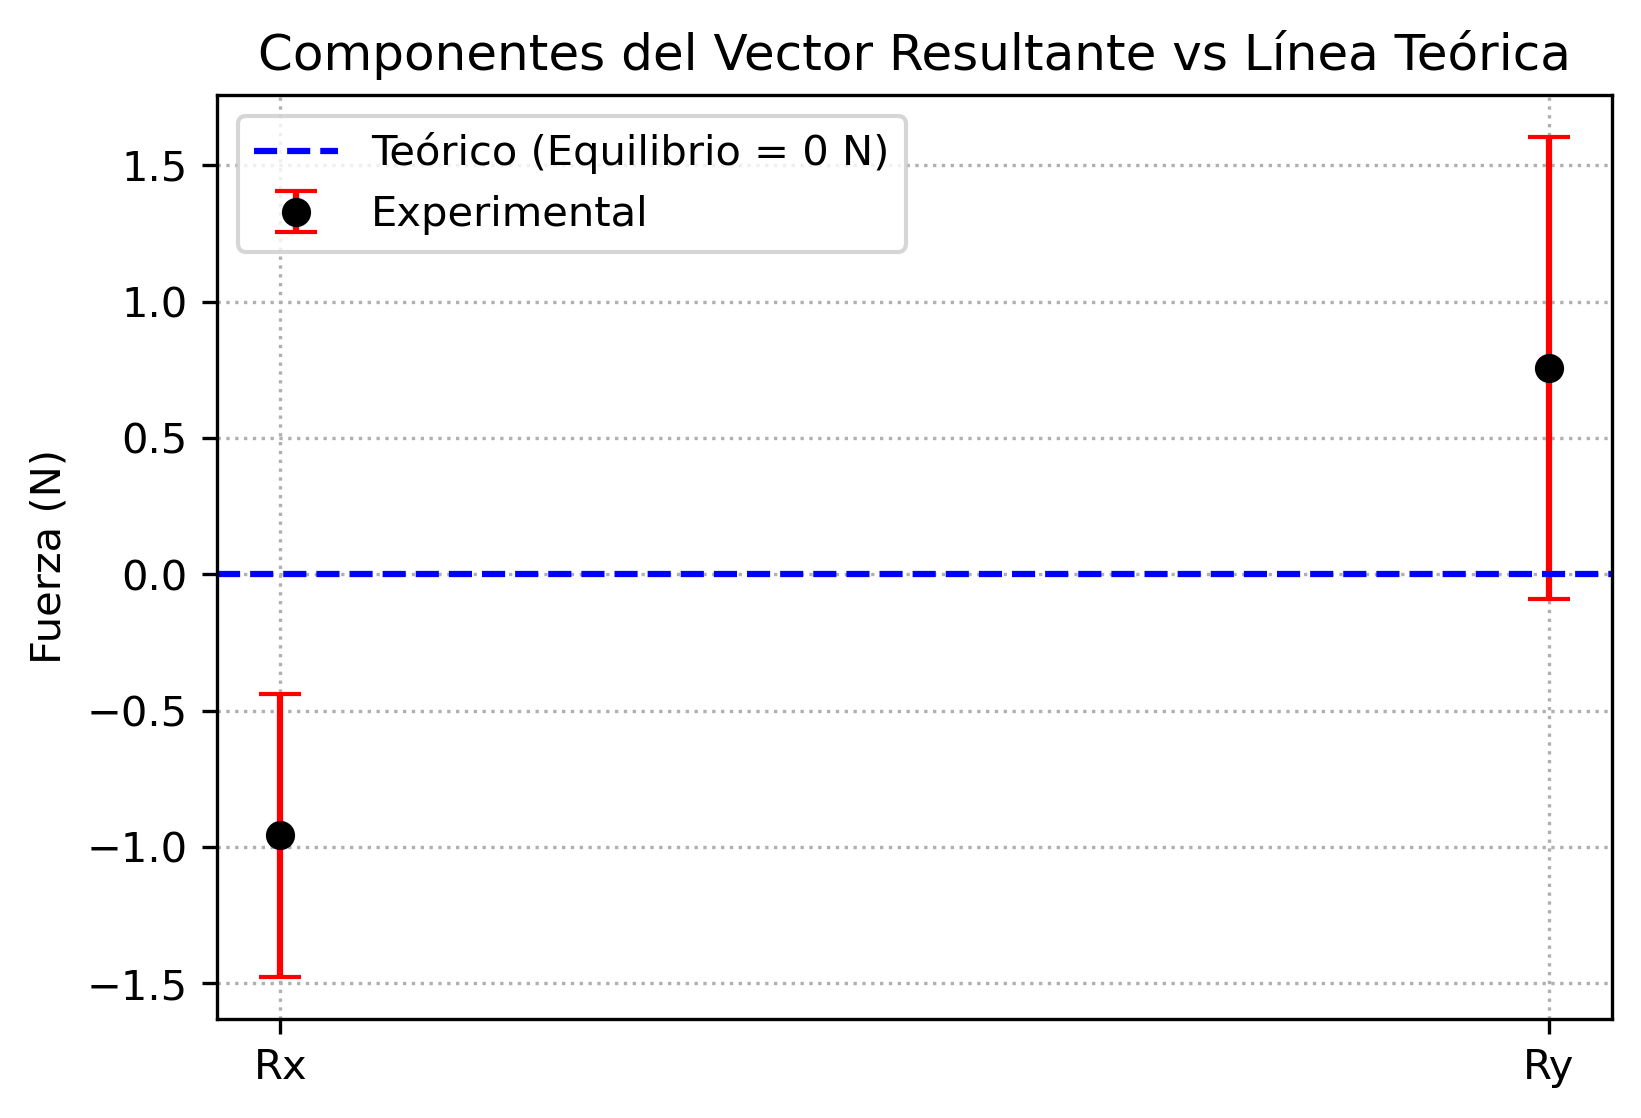
\includegraphics[width=0.4\textwidth]{grafico-error-config1.png}
\caption{Gráficos de las componentes de la fuerza resultante $R_x$ y $R_y$ con barras de error en relación a la referencia teórica $y=0\,\mathrm{N}$ para la Configuración 1.}
\label{fig:grafico-error-1}
\end{figure}Describan y analicen el gráfico obtenido. Indiquen si las barras de error de las componentes $R_x$ y $R_y$ cruzan la línea de referencia $y = 0\,\mathrm{N}$ y qué concluyen a partir de dicho cruce sobre la compatibilidad experimental con la condición de equilibrio traslacional.
